\documentclass{article}
\usepackage{graphicx} %package to manage images
\usepackage{hyperref}

\graphicspath{ {images/} }

\begin{document}
\section{Architecture}
Our project is split up in certain types of files which are part of one of the three layers:

This project layout lends itself well to a MVC-pattern. This can be seen in the following diagram:

\begin{figure}[h]
\centering
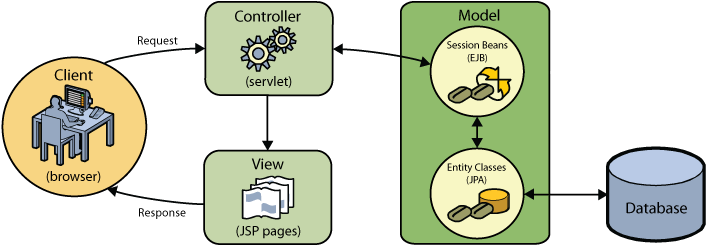
\includegraphics[width=0.75\textwidth]{mvc-diagram.png}
\small\textit{Source:\url{ https://netbeans.org/kb/docs/javaee/ecommerce/design.html}}
\end{figure}
\section{Functionalities}
Functionalities currently implemented are:

\begin{itemize}
\item \textbf{Registration:} A user can create an account. All the properties defined in the assignment are included.
\item \textbf{Login:} A user can use the account he created to log in. When a user logs in, a \textbf{session} will be created keeping the user logged in until he logs out or a timeout happens.
\item \textbf{Statistics:} When a user logs in, this gets saved into the database. On the statistics page a user can request the statistics about his login attempts.
\item \textbf{Settings:} A logged in user can access his settings and update them. (Currently all the settings except for the email)
\end{itemize}

\section{Implementation choices}
\subsection{Front-end}
We decided on using the jsp/servlet technology for the front-end and the request handling, because we were most familiar with those technologies and it seemed like they had the most complete information online.

\subsection{Beans}
The features we currently have don't require very complex interactions between the user and the beans. Most interactions consist of singular operations. Because of this, we are only using stateless beans right now. This will improve performance, especially when the amount of users grows exponentially.
\subsection{DBMS}
For our database management system we currently use derby. We are however considering switching to mysql because we are more familiar with mysql which may prevent future complexityproblems.
\end{document}